% 图 22.6 —— 由 `checks/emit_hand.py` 自动拼出（probe 精测 + prims2 图元分解）
%%
% ⚠ 这是**稿子不是成品**：跑 `checks/checkhand.py 22.6` 看指标 + 看叠合图。
%%
%% ⚠ 待核：
%   · 本图 probe 报出阴影族 1 个 —— **本脚本不生成阴影**（要照原书手写）；prims2 的 strokes 里可能含阴影线，核对时留意别画重
%   · 可疑字形 2 项（空心圈 ⊙ 常被认成字母 o）—— 见文件末
%%
\documentclass[12pt]{standalone}
\usepackage{fontspec}
\setsansfont{Arial}
\newfontfamily\mfallback{DejaVu Sans}
\usepackage{tikz}
\begin{document}
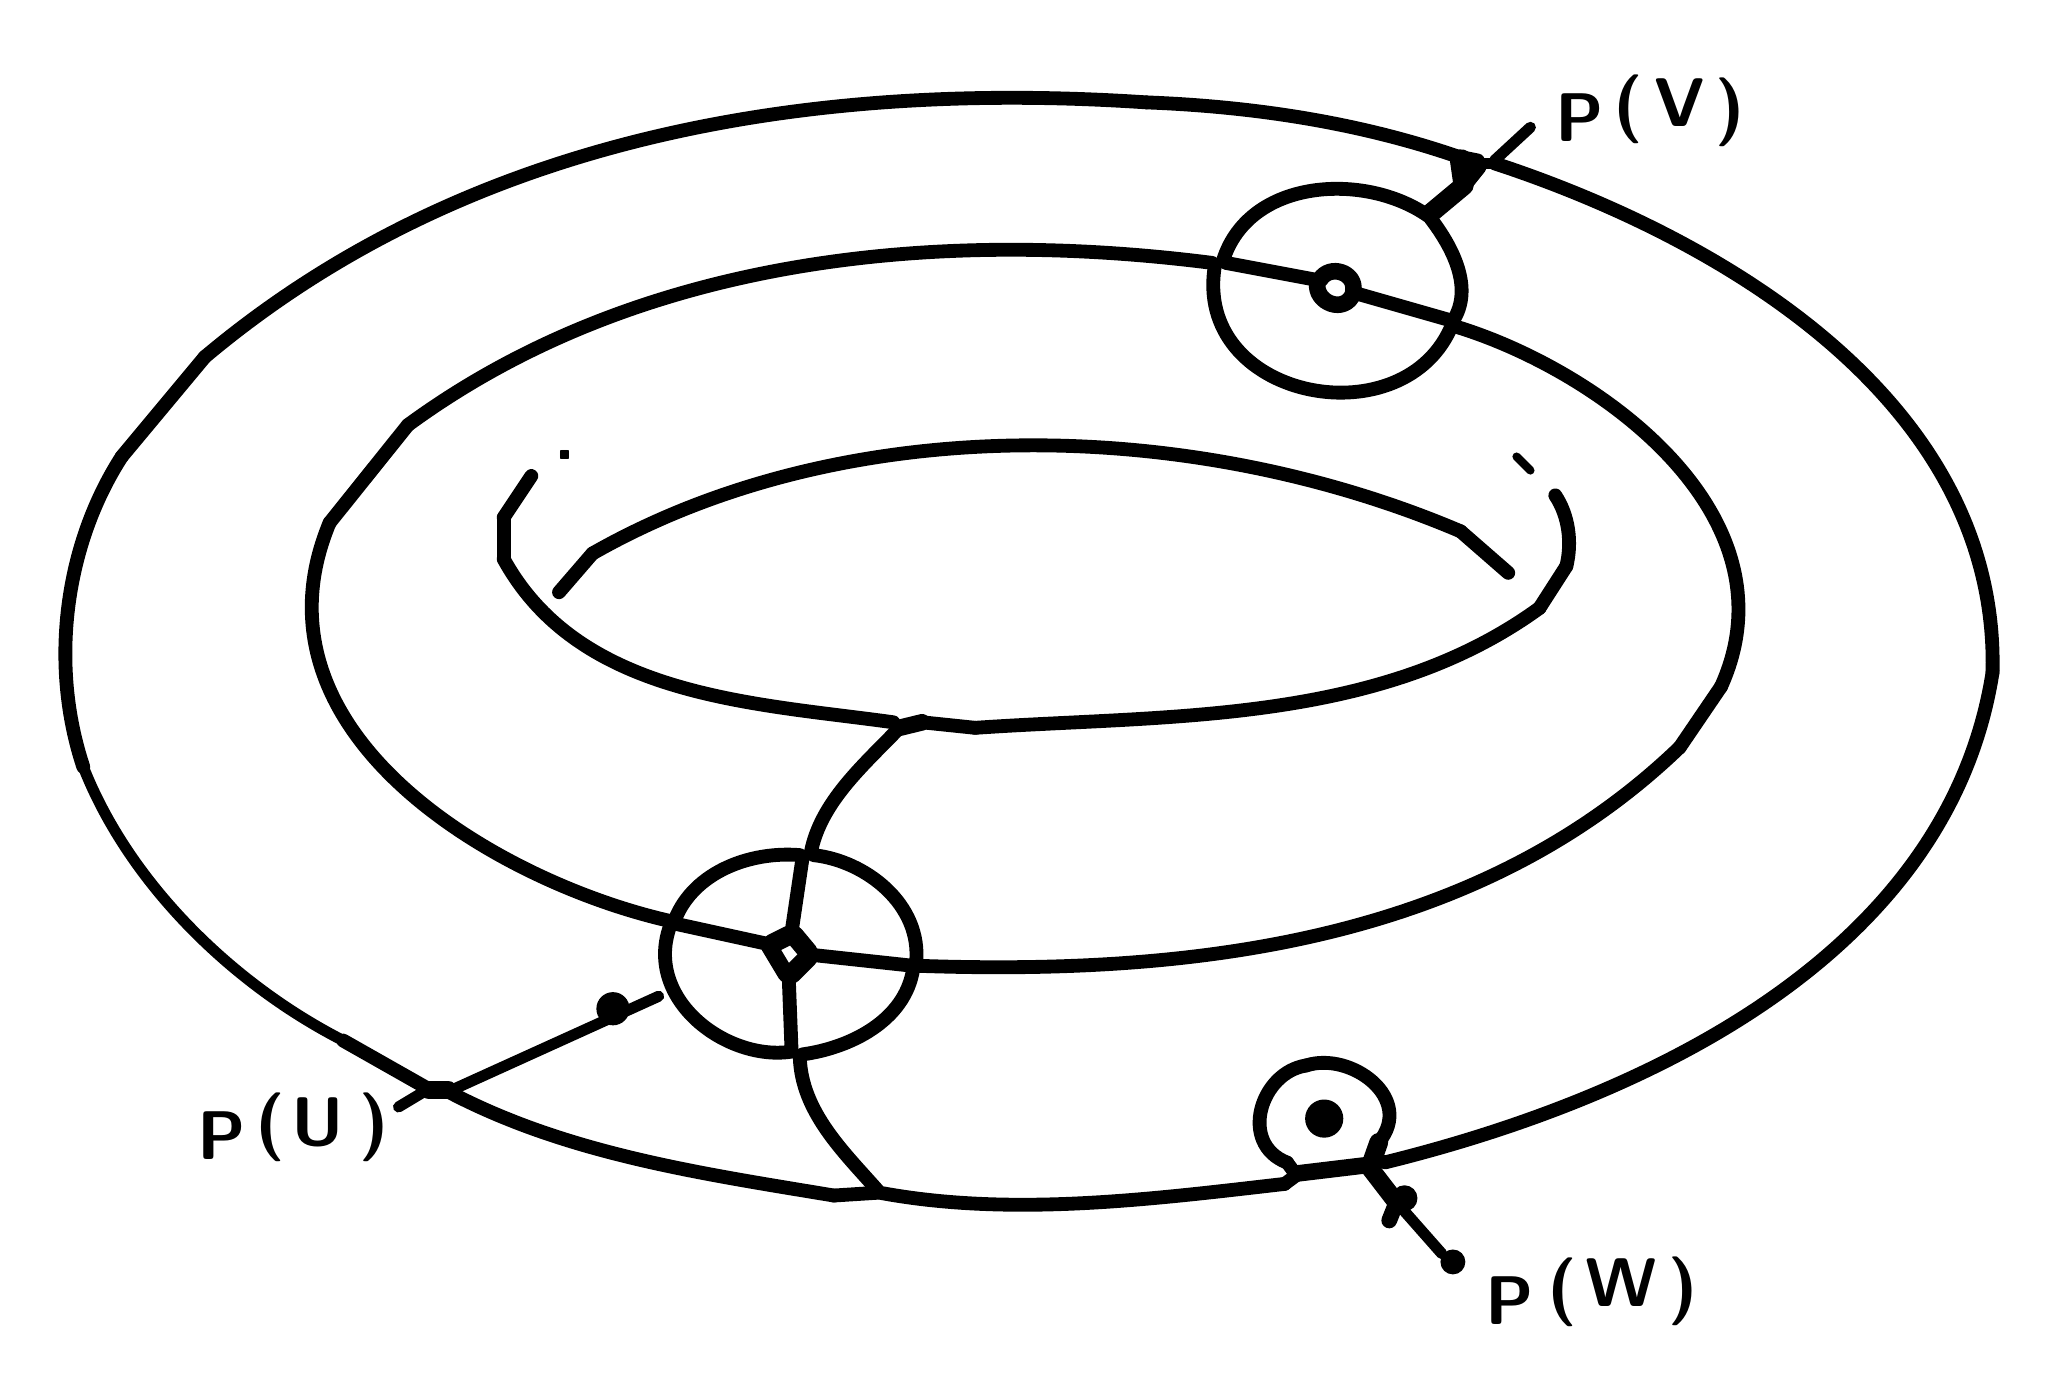
\begin{tikzpicture}[x=1pt, y=-1pt, line width=6.0pt, line cap=round, line join=round]

  %% ════ 填充区（prims2 的 fills）════

  %% ════ 直线段（prims2 的 strokes）════
  \draw[line width=6.0pt] (268.0,332.0) -- (274.0,342.0);
  \draw[line width=4.0pt] (511.0,443.0) -- (496.0,426.0);
  \draw[line width=4.0pt] (228.0,350.0) -- (153.0,384.0);
  \draw[line width=8.1pt] (518.0,48.0) -- (519.0,55.0);
  \draw[line width=5.0pt] (192.0,204.0) -- (204.1,190.0);
  \draw[line width=5.0pt] (517.8,182.0) -- (535.0,197.0);
  \draw[line width=7.0pt] (507.0,67.0) -- (519.0,57.0);
  \draw[line width=5.0pt] (519.0,47.0) -- (524.0,48.0);
  \draw[line width=6.0pt] (459.0,414.0) -- (484.0,411.0);
  \draw[line width=7.0pt] (275.0,328.0) -- (269.0,331.0);
  \draw[line width=3.0pt] (315.0,253.0) -- (312.8,251.0);
  \draw[line width=5.0pt] (172.0,192.0) -- (172.0,177.0);
  \draw[line width=5.0pt] (172.0,177.0) -- (182.0,162.0);
  \draw[line width=6.0pt] (315.0,253.0) -- (323.2,251.0);
  \draw[line width=5.0pt] (323.2,251.0) -- (342.4,253.0);
  \draw[line width=5.0pt] (546.3,209.7) -- (556.0,194.6);
  \draw[line width=5.0pt] (144.0,383.0) -- (114.0,366.0);
  \draw[line width=5.0pt] (34.0,155.0) -- (64.0,119.0);
  \draw[line width=5.0pt] (611.9,238.1) -- (597.0,260.0);
  \draw[line width=4.9pt] (490.6,410.0) -- (486.0,409.0);
  \draw[line width=7.0pt] (277.0,328.0) -- (282.0,334.0);
  \draw[line width=7.0pt] (276.0,342.0) -- (282.0,336.0);
  \draw[line width=5.0pt] (275.0,343.0) -- (276.0,369.0);
  \draw[line width=6.5pt] (520.0,55.0) -- (524.0,50.0);
  \draw[line width=5.7pt] (494.0,426.0) -- (492.0,431.0);
  \draw[line width=4.0pt] (525.0,49.0) -- (529.0,49.0);
  \draw[line width=6.5pt] (152.0,384.0) -- (145.0,384.0);
  \draw[line width=4.9pt] (454.2,417.8) -- (458.0,415.0);
  \draw[line width=4.9pt] (458.0,414.0) -- (455.1,410.1);
  \draw[line width=6.8pt] (488.2,402.8) -- (486.0,409.0);
  \draw[line width=5.0pt] (320.0,339.0) -- (283.0,335.0);
  \draw[line width=5.0pt] (480.0,96.0) -- (515.0,106.0);
  \draw[line width=5.0pt] (465.0,91.0) -- (433.0,85.0);
  \draw[line width=3.0pt] (543.0,160.0) -- (538.0,155.0);
  \draw[line width=6.5pt] (495.0,425.0) -- (485.0,412.0);
  \draw[line width=4.0pt] (543.0,36.0) -- (530.0,48.0);
  \draw[line width=5.0pt] (235.0,324.0) -- (267.0,331.0);
  \draw[line width=4.0pt] (134.0,390.0) -- (144.0,384.0);
  \draw[line width=5.0pt] (280.0,300.0) -- (276.0,327.0);
  \draw[line width=5.0pt] (137.4,143.6) -- (109.1,178.9);
  \draw[line width=5.0pt] (307.0,421.0) -- (291.3,422.0);

  %% ════ 曲线（prims2 的 curves —— 三段式，坐标同为 (y,x)）════
  \draw[line width=5.0pt] (429.0,86.0) .. controls (421.0,133.7) and (495.5,148.9) .. (514.0,109.0);
  \draw[line width=5.0pt] (204.1,190.0) .. controls (296.3,137.5) and (421.5,141.0) .. (517.8,182.0);
  \draw[line width=5.0pt] (279.0,372.0) .. controls (279.6,391.7) and (294.8,406.2) .. (307.0,420.0);
  \draw[line width=5.0pt] (280.0,371.0) .. controls (296.9,368.7) and (317.1,359.0) .. (320.0,340.0);
  \draw[line width=5.0pt] (312.8,251.0) .. controls (262.6,244.0) and (199.5,242.1) .. (172.0,192.0);
  \draw[line width=5.0pt] (342.4,253.0) .. controls (412.2,248.2) and (488.1,252.0) .. (546.3,209.7);
  \draw[line width=5.0pt] (556.0,194.6) .. controls (558.1,186.0) and (556.9,176.4) .. (552.0,169.0);
  \draw[line width=5.0pt] (315.0,253.0) .. controls (302.3,266.3) and (286.6,279.6) .. (283.0,298.0);
  \draw[line width=4.0pt] (114.0,366.0) .. controls (74.1,345.6) and (36.7,309.3) .. (20.1,267.1);
  \draw[line width=5.0pt] (20.1,267.1) .. controls (7.8,230.2) and (13.3,187.1) .. (34.0,155.0);
  \draw[line width=5.0pt] (64.0,119.0) .. controls (158.3,39.7) and (281.4,18.8) .. (404.3,27.0);
  \draw[line width=5.0pt] (404.3,27.0) .. controls (443.7,28.5) and (482.2,34.5) .. (518.0,47.0);
  \draw[line width=5.0pt] (516.0,108.0) .. controls (567.8,123.7) and (640.0,176.1) .. (611.9,238.1);
  \draw[line width=5.0pt] (597.0,260.0) .. controls (524.0,330.3) and (421.4,342.4) .. (322.0,339.0);
  \draw[line width=5.0pt] (234.0,322.0) .. controls (240.9,305.1) and (261.0,297.5) .. (279.0,299.0);
  \draw[line width=5.0pt] (530.0,49.0) .. controls (610.7,75.5) and (712.4,134.0) .. (710.0,233.0);
  \draw[line width=5.0pt] (710.0,233.0) .. controls (693.6,337.2) and (580.9,387.7) .. (490.6,410.0);
  \draw[line width=5.0pt] (276.0,370.0) .. controls (252.8,373.6) and (222.8,351.4) .. (232.0,325.0);
  \draw[line width=5.0pt] (308.0,421.0) .. controls (355.7,429.9) and (407.0,423.2) .. (454.2,417.8);
  \draw[line width=6.0pt] (479.0,95.0) .. controls (480.0,88.4) and (470.5,85.3) .. (467.0,91.0);
  \draw[line width=5.0pt] (455.1,410.1) .. controls (437.5,403.3) and (445.4,377.5) .. (462.0,375.0);
  \draw[line width=5.0pt] (462.0,375.0) .. controls (478.1,369.8) and (501.4,386.9) .. (488.2,402.8);
  \draw[line width=5.0pt] (284.0,299.0) .. controls (302.8,301.0) and (323.3,316.9) .. (321.0,338.0);
  \draw[line width=5.0pt] (515.0,106.0) .. controls (522.8,93.9) and (514.6,79.0) .. (507.0,69.0);
  \draw[line width=5.0pt] (506.0,68.0) .. controls (483.5,52.2) and (441.5,54.2) .. (432.0,84.0);
  \draw[line width=6.0pt] (466.0,92.0) .. controls (464.9,99.6) and (476.1,103.7) .. (479.0,96.0);
  \draw[line width=5.0pt] (428.0,85.0) .. controls (326.7,72.1) and (219.4,83.5) .. (137.4,143.6);
  \draw[line width=5.0pt] (109.1,178.9) .. controls (77.1,255.7) and (171.4,309.4) .. (233.0,323.0);
  \draw[line width=5.0pt] (291.3,422.0) .. controls (243.8,414.1) and (195.7,407.2) .. (153.0,385.0);

  %% ════ 实心点 ════
  \fill (468.5,394.2) circle (6.9);
  \fill (211.5,354.5) circle (6.0);
  \fill (497.5,423.0) circle (4.7);
  \fill (515.0,446.0) circle (4.5);

  %% ════ 标签（probe 直接给的 \node 行）════
  %% ⚠ 全部补了 fill=white：文字在最上层，否则与曲线交叉干扰
     \node[anchor=center,inner sep=0pt,fill=white,font=\fontsize{30.7}{38.4}\selectfont] at (578.5,29.5) {\textsf{\textbf{(}}};   % box(574,15,8,28)
     \node[anchor=center,inner sep=0pt,fill=white,font=\fontsize{28.0}{35.0}\selectfont] at (597.3,26.9) {\textsf{\textbf{\textit{V}}}};   % box(589,15,17,22)
     \node[anchor=center,inner sep=0pt,fill=white,font=\fontsize{32.6}{40.7}\selectfont] at (615.1,30.5) {\textsf{\textbf{)}}};   % box(609,16,9,28)
     \node[anchor=center,inner sep=0pt,fill=white,font=\fontsize{29.8}{37.3}\selectfont] at (561.0,32.5) {\textsf{\textbf{\textit{P}}}};   % box(550,20,18,23)
     \node[anchor=center,inner sep=0pt,fill=white,font=\fontsize{33.5}{41.9}\selectfont] at (194.0,154.3) {\textsf{\textbf{.}}};   % box(189,152,5,4)
     \node[anchor=center,inner sep=0pt,fill=white,font=\fontsize{30.7}{38.4}\selectfont] at (87.5,397.5) {\textsf{\textbf{(}}};   % box(83,383,8,28)
     \node[anchor=center,inner sep=0pt,fill=white,font=\fontsize{29.6}{37.0}\selectfont] at (105.0,395.2) {\textsf{\textbf{\textit{U}}}};   % box(95,383,20,22)
     \node[anchor=center,inner sep=0pt,fill=white,font=\fontsize{32.6}{40.7}\selectfont] at (125.1,397.5) {\textsf{\textbf{)}}};   % box(119,383,9,28)
     \node[anchor=center,inner sep=0pt,fill=white,font=\fontsize{29.8}{37.3}\selectfont] at (70.0,400.5) {\textsf{\textbf{\textit{P}}}};   % box(59,388,18,23)
     \node[anchor=center,inner sep=0pt,fill=white,font=\fontsize{29.9}{37.4}\selectfont] at (576.2,453.5) {\textsf{\textbf{\textit{W}}}};   % box(563,441,26,23)
     \node[anchor=center,inner sep=0pt,fill=white,font=\fontsize{32.6}{40.7}\selectfont] at (598.1,456.5) {\textsf{\textbf{)}}};   % box(592,442,9,28)
     \node[anchor=center,inner sep=0pt,fill=white,font=\fontsize{30.2}{37.7}\selectfont] at (554.5,457.0) {\textsf{\textbf{(}}};   % box(550,443,8,27)
     \node[anchor=center,inner sep=0pt,fill=white,font=\fontsize{30.0}{37.4}\selectfont] at (535.5,460.0) {\textsf{\textbf{\textit{P}}}};   % box(524,448,19,22)

  % 钉死画布：否则超出的图元/控制点会把页面撑大，1:1 回比就失准
  \pgfresetboundingbox
  \path[use as bounding box] (0,0) rectangle (721,478);
\end{tikzpicture}
\end{document}

% ⚠ 待核清单（probe 拿不准，人眼过一遍）：
%   · 未识别/跳过：⑤ 跳过/未识别的字形
%   · 未识别/跳过：box(538,155,7,7)
